\newpage

\chapter{2D Flow Around a Cylinder}

SPARTA has built-in support for 2D simulations. Additionally, it also has the ability to render particles and surfaces in the simulation through ray tracing at any instant of time. These features have been utilized and are discussed in this chapter.

\section{Setup}

The setup for the simulation is represented in Figure \ref{img:flow}.

\begin{figure}[H]
  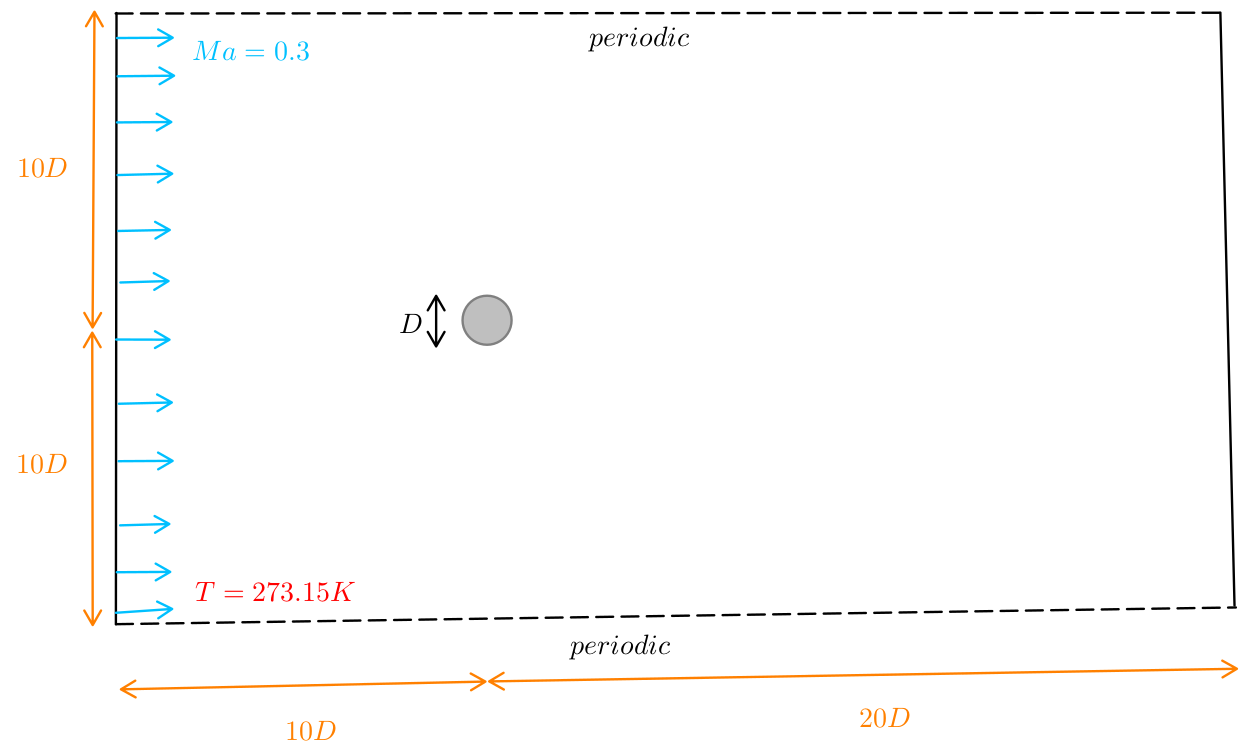
\includegraphics[scale=0.3]{Pictures/Chapter_6_2D_Flow/Flow.png}
  \centering
  \caption{Setup of the simulation}
  \label{img:flow}
\end{figure}

\no There is a circular cylinder of diameter $D = 0.01 m$ placed in the flow and the domain selected to be large in comparison to the cylinder to reduce boundary effects in the simulation. The extent of the domain behind the cylinder is longer than the domain ahead as the wake that is formed behind a cylinder is often quite complex and is of more interest in general. The flow at the inlet is set to be at a uniform $Ma = 0.3$ where compressibility effects just start to appear and the temperature is kept at 273.15 K throughout the inlet. \\

\no The hierarchical grid that SPARTA provides is utilised in this simulation, where there 	$(30 \times 20 \times 1)$ grid cells in the first level called the \textit{sampling cells}. These sampling cells are used to sample the macroscopic properties such as temperature and pressure throughout the domain. However, these cells are too large for there to be accurate collision statistics within them, so each sampling cell is further divided into $(2 \times 2 \times 1)$ \textit{collision cells}. Each of these collision cells has about 62.5 particles in them. The simulation ratio $F_N$ is taken to be $6.72 \times 10 ^{14}$ and this yields $N = 1.01 \times 10^{20}$. If we account for the volume of the simulation domain and use Equation \ref{eq:mean_free_path} to calculate the mean free path as $\lambda = 0.001$ when we consider the gas to be Argon. Using Equation \ref{eq:kn}, we can calculate the Knudsen number of the simulation to be about 0.1. Since the Knudsen number and the Mach number of the flow are known, the Reynolds number can be found using,

\begin{equation}
	Kn = \frac{Ma}{Re} \sqrt{\frac{\gamma \pi}{2}}
\end{equation}

\no From the above equation, we obtain $Re \approx 4.59$. We also obtain the mean collision time from Equation \ref{eq:mean_coll_time} as $t_o \approx = 3 \times 10 ^ {-6} s$ and hence the time step is chosen to be $\tau = 3 \times 10 ^ {-7} s$ and the simulation is performed for a million timesteps, yielding a total physical time of 0.3 s.

\section{Ray Traced Images}

This section gives some ray-traced images given by SPARTA. These images can be output for any simulation, from any orientation, and serve as a valuable way to visualize the flow. The images for every timestep can be found in \cite{Raghuveeran_Work_During_Summer_2024}. \\

\no Figure \ref{img:wake} gives an image of the flow at the $950,000^{th}$ step of the simulation. One can observe that the particles seem to be closer to each other before the cylinder than they are after. We can infer this as the region before the cylinder has a lot more red spots than the region after.

\begin{figure}[H]
  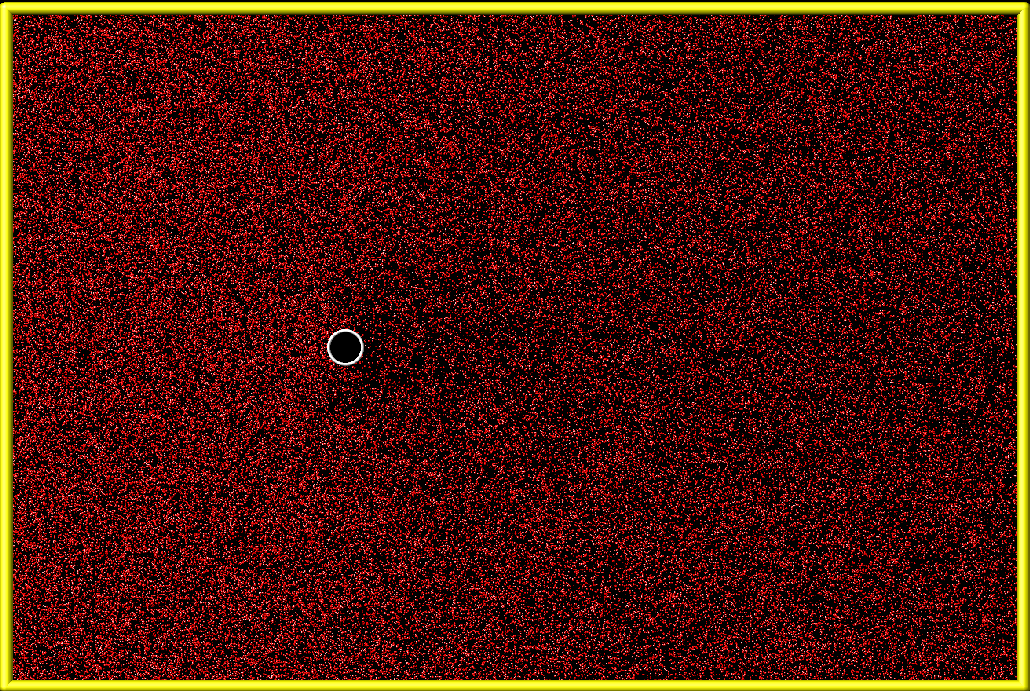
\includegraphics[scale=0.4]{Pictures/Chapter_6_2D_Flow/dump.png}
  \centering
  \caption{Ray Traced Image of the Flow}
  \label{img:wake}
\end{figure}

\no It can be seen that the region behind the cylinder has fewer particles than the region in front. This is a very crude representation of the wake that is formed behind the cylinder under these flow conditions. \\

\no Apart from these observations, since the flow at the inlet is uniform and the cylinder is placed symmetrically about the vertical extents of the domain, we can expect the flow to be symmetric. If the flow is symmetric, then we expect the lift to be zero around the cylinder while the drag is along the positive $x$-direction. Figures \ref{gra:lift} and \ref{gra:drag} show exactly that.

\begin{figure}[H]
	\centering
    \includesvg[width=0.6\linewidth]{Pictures/Chapter_6_2D_Flow/Lift.svg}
    \caption{Lift variation with time}
	\label{gra:lift}
\end{figure}

\no Notice how in Figure \ref{gra:lift} the average lift is nearly 0 while in Figure \ref{gra:drag}, the average drag is orders of magnitude higher and non-zero. One can also see the transience as drag increases from zero to its steady-state value near the beginning of the simulation.

\begin{figure}[H]
	\centering
    \includesvg[width=0.6\linewidth]{Pictures/Chapter_6_2D_Flow/Drag.svg}
    \caption{Drag variation with time}
	\label{gra:drag}
\end{figure}